\subsection{Event dispatching}
\label{sec:eventdispatch}
We've decided to create a system that handles the dispatching of events. This 
system looks a lot like an Observer Pattern. Instead of registering observers 
to a subject, we register slots and uicomponents to the event dispatcher.
This EventDispatcher class then decides in its dispatch method where to send 
the event to. We've done this so that when, for example, we move the mouse 
on the world panel, we don't call the other panel's callback function.
What the event dispatcher looks like and its relation with ui components and 
slots are shown in \cref{fig:eventdispatcher}.

\begin{figure}[H]
\centering
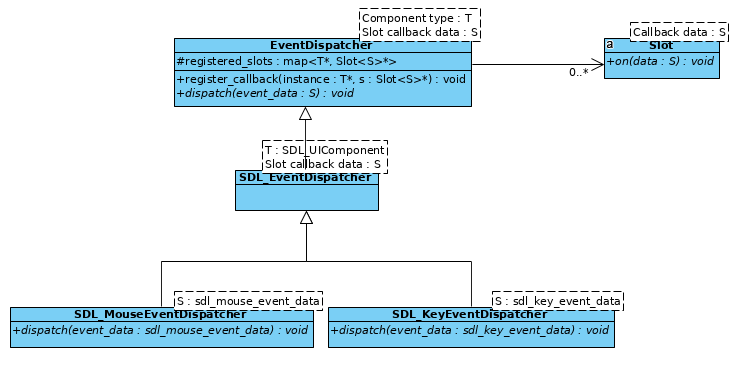
\includegraphics[scale=0.6]{res/events/eventdispatch.png}
\caption{The EventDispatcher and derived classes}\label{fig:eventdispatcher}
\end{figure}

\subsubsection{Deciding the right panel}
\label{sec:eventdispatcher-dispatch}
As we've mentioned before, when we send an event, we don't want to call each 
panel's callback slot. We needed to create some logic for deciding where to 
send the event, which can be seen in \cref{lst:sdleventdispatch}.
\\

\begin{lstlisting}[caption={SDL\_MouseEventDispatcher dispatch method.},
label={lst:sdleventdispatch}]
void SDL_MouseEventDispatcher::dispatch(sdl_mouse_event_data d) {
    SDL_UIComponent *best_component = nullptr;
    Slot<sdl_mouse_event_data> *best_slot = nullptr;
    for (std::map<SDL_UIComponent *, Slot<sdl_mouse_event_data> *>::iterator it = _registered_slots.begin();
         it != _registered_slots.end(); ++it) {
        SDL_UIComponent *current_component = (*it).first;
        float current_distance = current_component->get_position()->distance(d.position);
        if (current_component->contains_point(d.position) &&
            (!best_slot || current_distance < best_component->get_position()->distance(d.position))) {
            best_component = current_component;
            best_slot = (*it).second;
        }
    }
    if (best_slot) {
        d.component = best_component;
        best_slot->on(d);
    }
}
\end{lstlisting}
